Researchers have been studying confinement for decades~\cite{lampson1973_confinement}, and
have been designing and applying confinement primitives since the early days of
time-sharing computers and multi-tenant systems~\cite{shu2016_security_isolation_study}.
While many developments have been made in the mean time, the current confinement
landscape (particularly within the Linux ecosystem) suffers from a few fundamental flaws
that culminate in poor container security practices; this does not need to be so. This
chapter presents a critique of the current state of confinement on Linux, examines how
confinement primitives are applied to containers, and proposes a fundamental re-framing of
the problem to focus on \todo{WHAT THREE THINGS?}. In light of this re-framing, we
consider design goals for \bpfbox{} and \bpfcontain{} and present the threat model for
confinement under these research systems.

\section{Rethinking the Virtualization Narrative}%
\label{s:cp-rethinking}

Hypervisor-backed virtualization is commonly considered more secure than
con\-tain\-er-based virtualization~\cite{sultan2019_container_security,
eder2016_hypervisor_container}.  Intuitively, this makes sense. Containers run directly on
the host operating system, whereas a virtual machine runs on top of a hypervisor,
separated by at least one layer of indirection from the host system. However, this
intuition does not strictly stand up to scrutiny. A virtual machine running on top of
a hypervisor makes requests to the hypervisor's \gls{api} (via hypercalls), in much the
same way as a container running on a host operating system makes requests to the kernel's
\gls{api} (via system calls).  \Cref{fig:syscall-hypercall} illustrates this parity.

\begin{figure}[htbp]
  \centering
  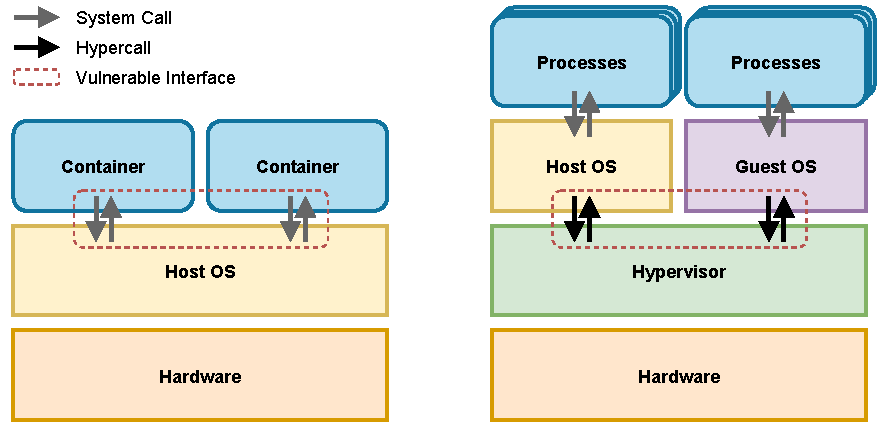
\includegraphics[width=0.8\linewidth]{figs/confinement-problem/syscall-hypercall.pdf}
  \caption[System calls and hypercalls as vulnerable interfaces]{
    System calls and hypercalls as vulnerable interfaces. Containers (which are really
    just process groups running on the host \gls{os}) make system calls to the
    more-privileged host \gls{os} kernel. Similarly, a guest operating system makes
    hypercalls to the more-privileged hypervisor. Both of these interfaces are ripe
    targets for a myriad of attacks, including privilege escalation and tampering with
    sensitive resources. This parity becomes particularly evident when we assume that an
    attacker has or is able to obtain control over the guest \gls{os}.
  }%
  \label{fig:syscall-hypercall}
\end{figure}

The isolation guarantees provided by a virtual machine come almost entirely from a sense
of obfuscation over a semantic gap, created as the hypervisor virtualizes system
resources. There is no notion of centralized policy in a virtual machine; rather, security
is an emergent phenomenon, a form of \enquote{policy through mechanism}. With the right
tools, we can and have poked holes everywhere in this
policy~\cite{dubrelle2015_hypervisor, thongthua2016_analysis, shahzad2017_systematic}.

The central argument of this thesis is that there is no fundamental reason why containers
cannot be as\,---\,if not more\,---\,secure than virtual machines. While it is true that
a containerized process is nothing more than a host process running under some virtualized
state, an operating system that provides and enforces the right set of confinement
primitives should be able to lock a container down in much the same way that a hypervisor
implicitly enforces isolation. Unlike hypervisor-based isolation, a policy enforced by the
operating system has the potential to be more minimal, centralized, and accessible to
end-users. The key to developing such an enforcement mechanism lies in defining a clear
protection boundary within the kernel and enforcing access across this boundary. \bpfbox{}
lays the foundation for such an enforcement mechanism, and \bpfcontain{} explicitly
applies it to containers.

In \bpfbox{}, policies are defined in a centralized, flexible policy file. Using
\gls{ebpf}, \bpfbox{} can observe various aspects of system behaviour, such as user and
kernelspace function calls, and incorporate them into its enforcement decisions. This
helps define fine-grained policy while keeping the overall policy syntax clean and simple.
\bpfcontain{} extends this model by defining an implicit protection boundary around
a container, where the container is made up of a set of host processes and associated
resources. Operations \textit{within} the container are implicitly allowed, whereas
operations \textit{outside} the container or operations that can affect the system as
a whole are implicitly denied. In this way, \bpfcontain{} policy allows the user to define
\textit{exceptions to implicit rules} rather than the rules themselves.

The key insight behind both \bpfbox{} and \bpfcontain{} is that novel kernel mechanisms
are required to realize their respective goals. The new \gls{ebpf} kernel technology
provides precisely the right framework for developing such mechanisms. In \bpfcontain{},
a clear and well-defined abstraction for containers allows the kernel to enforce implicit
policy centred around container semantics. We rely on \gls{ebpf} to enable the definition
of such an abstraction without necessarily tying the kernel down to one specific
interpretation of what a container actually is. Using multiple \gls{ebpf} programs and
maps, we can combine various other aspects of system behaviour with \gls{lsm}-based
enforcement in a stateful manner. \bpfbox{} uses its ability to introspect system state to
enable policy enforcement at the granularity of individual function calls.

At this point, it should be clear that both \bpfbox{} and \bpfcontain{} leverage the power
of \gls{ebpf} to make improvements on the existing status quo of Linux confinement. The
next two sections, \Cref{s:cp-issues} and \Cref{s:cp-containers}, discuss the state of
confinement on Linux and how existing container technologies apply confinement primitives.
This discussion serves to contextualize the notions behind this section and motivates the
need for \bpfbox{} and \bpfcontain{} as novel confinement primitives.

% \begin{inprogress}
%   \begin{itemize}
%     \item Just like the word container makes people think about security
%     \item Type I and Type II hypervisor, the way it's depicted, makes people think something else is happening
%     \item The representation and terminology
%     \item This makes sense to talk about it if we connect it to containers
%     \item Why can't containers give as good or better security than hypervisors
%     \item Can we just get our enforcement clear
%     \item Virtual machines seem like they define a clear boundary, but it isn't actually
%           so clear in practice because all these things are being shared across boundaries
%     \item People think of virtual machines as being inherently more secure, the security
%           benefit is more of an obfuscation thing related to the semantic gap but with the right
%           tools you can still cross it freely
%     \item VMs have all these little holes everywhere and the policy is not centralized\,---\,we
%           have policy through mechanism
%     \item There's no reason why containers can't be as (if not more) secure than virtual machines
%     \item Because we can make this boundary very clear
%     \item \bpfcontain{} can be seen as a step towards this
%   \end{itemize}
% \end{inprogress}



\section{Fundamental Issues with Linux Confinement}%
\label{s:cp-issues}

\begin{enumerate}
  \item \textbf{Complexity and Interdependence.}
    Existing confinement primitives are overly complex and designed for use
    cases beyond simple process confinement. This results in a pattern of
    abusing existing mechanisms
  \begin{inprogress}
    \begin{itemize}
      \item Existing confinement solutions are overly complex
      \item Based on a number of low-level primitives that were originally designed for
            totally different tasks.
      \item Namespaces were designed to virtualize resources. They provide a form of
            isolation but not confinement; need a way to deal with namespace escapes
      \item Cgroups, similarly, were designed to virtualize the availability of system
            resources, not to directly confine.
      \item Unix \gls{dac} is far too coarse-grained and easy to bypass to be practically useful for confinement.
      \item POSIX capabilities can be used to reduce overprivilege by portioning root privileges, but do not
            implement confinement by themselves.
      \item Seccomp-bpf works well to reduce the availability of system calls, but writing
            classic \gls{bpf} filters is complex and error-prone. Anything beyond basic system call
            filtering quickly becomes untenable, particularly considering race conditions when
            checking arguments.
    \end{itemize}
  \end{inprogress}

  \item \textbf{\todo{WHAT GOES HERE}.}
  \begin{inprogress}
    \begin{itemize}
      \item
    \end{itemize}
  \end{inprogress}

  \item \textbf{Difficulty Adopting New Solutions.}
  \begin{inprogress}
    \begin{itemize}
      \item Motivated by the above difficulties, academics are often tempted to propose new confinement solutions.
      \item Many try to solve the problem by simply recombining and reusing these existing primitives in new ways.
      \item This isn't really a step forward, as we are still subject to limitations introduced in item 1 and item 2.
      \item To really solve the problem, we need kernel-level support for something new.
      \item The issue is that new solutions based on kernel support are not necessarily
            adoptable. New kernel code can introduce bugs and security vulnerabilities, and
            needs to be thoroughly tested before it can be considered production-ready.
      \item Another problem arises when we consider container-specific confinement as an
            end goal; not everyone can agree on what the definition of a \enquote{container}
            even is, so how can we hope to reach agreement on what a new abstraction for
            container-based confinement would even look like.
      \item To solve this problem, we need a way to add new abstractions to the kernel in
            a way that is neither binding nor limited by the lack of adoptability associated
            with traditional kernel-based solutions.
    \end{itemize}
  \end{inprogress}
\end{enumerate}



\section{How Containers Apply Confinement Primitives}%
\label{s:cp-containers}

This section examines and critiques the way Linux container technologies apply confinement
primitives to lock down container deployments. We focus primarily on Docker as a case
study, however these principles in general apply the majority of container management
frameworks.

In general, Linux containers have three broad goals. However, these goals are not
equally met by existing container management frameworks. In order of decreasing
prioritization, they are:
\begin{enumerate}
  \item \textbf{Dependency Management / Reproducibility.}
    Containers should provide an easy and robust framework for creating reproducible
    development environments. Dependencies should be maximally self-contained such that
    a containerized environment \enquote{just works} to the maximum possible extent. We
    can see examples of this property in Docker, the predominant container framework to
    date. Docker Hub~\cite{docker_hub} allows container images to be pulled from the
    Internet, recombined, and used to create further images. The end result is a flexible
    framework for creating and distributing reproducible development environments.

  \item \textbf{Virtualization.}
    Containers should virtualize system resources, creating the illusion of running on
    a separate physical machine. Where possible, resources should be transparently reused
    between multiple containers (e.g.~sharing a single base copy of the same shared
    library between two container images). To achieve virtualization, containers generally
    rely on the namespaces and cgroups primitives provided by the Linux kernel. Overlay
    filesystems~\cite{overlayfs} combined with the mount namespace aid containers one-way
    sharing of filesystem resources.

  \item \textbf{Confinement.}
    Containerized processes should be confined by default. That is, a containerized
    process should have access to the minimal set of privileges required for it to operate
    normally. The extent to which this property is achieved by conventional container
    frameworks varies greatly, both by framework and by individual
    deployment~\cite{sultan2019_container_security, lin2018_container_security,
    bui2015_docker_analysis}. In general, proper confinement is not a priority of
    container frameworks, and this tends to result in sacrificing security for
    ease-of-deployment.
\end{enumerate}

The aforementioned goals are not only ordered by their decreasing prioritization in extant
container management frameworks; they are also ordered by increasing relevance to
container security. That is to say, existing frameworks generally prioritize goals
unrelated to security and leave security as an afterthought. Since containers are really
just process groups running directly on the host operating system, an unconfined container
therefore exposes the same attack surface as an ordinary host process. Thus, one might
expect container security to be of paramount importance. Unfortunately, this is not the
case. These difficulties in confinement motivate the need to revisit container security
and approach it from a confinement-first perspective. To understand how these confinement
issues impact containers, we briefly review how container management systems apply
confinement primitives in practice.

To achieve confinement in the first place, container frameworks cobble together existing
confinement technologies and apply them ways that are often simultaneously confusing and
difficult to audit. The result is a complex policy soup with little room for customization
or auditability. For instance, Snap~\cite{snap} uses a high-level policy language that
targets system interfaces in a coarse-grained manner. Under the hood, this is compiled
into hundreds or thousands of lines of seccomp-bpf and AppArmor policy.
Docker~\cite{docker_security, docker_default_apparmor, docker_apparmor} uses a generic
AppArmor, seccomp-bpf, and POSIX capability policy for every container, along with default
namespace and control group configurations. Making meaningful changes to these policy
configurations, beyond simply disabling them altogether, is difficult and
error-prone~\cite{lin2018_container_security}.

Container security policies are often overly-generic and ill-suited to fine-grained
confinement. Part of the problem here is that containers in general are designed to
\enquote{just work}. Overly fine-grained security policies may get in the way of this,
particularly as end-user requirements vary and evolve across deployments.
Docker~\cite{docker_security}, for instance, provisions an overly-permissive default
AppArmor policy~\cite{docker_default_apparmor} designed to enforce basic protections
against interacting with sensitive kernel parameters without impacting the functionality
of the container. \todo{More examples}

Even worse, many container management systems operate under a fail-open approach when the
necessary security mechanisms are not supported. This results in low-security deployments,
often without even notifying the user that there may be such a configuration. Since the
end-user generally doesn't even participate in the policy authorship process, they may not
even be aware of the level of protection that is being applied, resulting in a dangerous
false sense of security. Docker's AppArmor policy~\cite{docker_apparmor,
docker_default_apparmor}, for instance, is not applied when the deployment environment
doesn't support AppArmor or AppArmor is disabled. Snap~\cite{snap} and others that rely on
the AppArmor or SELinux \glspl{lsm} for confinement suffer from similar failings.

Other aspects of confinement policy may be ignored entirely or even worse, overridden by
a more permissive policy, possibly without the user's knowledge.
Docker~\cite{docker_security} applies a dangerously permissive iptables policy that can
transparently expose a container to an external network, even overriding existing deny
rules. This overly-permissive network policy was the direct cause of a recent data breach
at NewsBlur~\cite{newsblur}, a news aggregation website, although NewsBlur administrators
claim that no user data was actually compromised~\cite{newsblur}. \todo{More examples}



\section{Design Goals}%
\label{s:cp-design}

Using the above analysis of the confinement problem, we can derive a clear set of design
goals for \bpfbox{} and \bpfcontain{}, such that they approach a solution to issues that
plague the status quo. In particular, we derive the following three design principles.
Note that these design principles are each the polar opposite of the three major problems
identified in \Cref{s:cp-issues}.

\begin{enumerate}
  \item \textbf{Simplicity and Flexibility.}
  \begin{inprogress}
    \begin{itemize}
      \item
    \end{itemize}
  \end{inprogress}

  \item \textbf{Sensible Defaults.}
  \begin{inprogress}
    \begin{itemize}
      \item
    \end{itemize}
  \end{inprogress}

  \item \textbf{Adoptability.}
  \begin{inprogress}
    \begin{itemize}
      \item
    \end{itemize}
  \end{inprogress}
\end{enumerate}





\section{The \bpfbox{} and \bpfcontain{} Threat Model}%
\label{s:cp-threat-model}

This section outlines the threat model for \bpfbox{} and \bpfcontain{}. In particular, we
provide a scoping definition of confinement policy and what it means for a policy
enforcement mechanism to confine a subject using that policy. We also discuss the
adversary's capabilities, goals, and potential attack vectors in a commodity Linux-based
operating system. In general, both \bpfbox{} and \bpfcontain{} have a very similar threat
model, with subtle and specific differences arising in a few key areas. Where
discrepancies arise, they will be noted accordingly.

\subsection{Confinement Policy}

We define \textit{confinement} as the restriction of \textit{subject} (system actors such
as processes) behaviours to a set of desired behaviours, as they pertain to
\textit{objects} (system resources such as files, network sockets, devices, and IPC
handles onto other subjects). Consider the set of all subjects $\mathcal{S}$ and the set
of all objects $\mathcal{O}$. We define $\mathcal{S} \subseteq \mathcal{O}$ to account for
IPC objects. The goal is to create a confinement policy $\mathcal{P}_i$ for a subject
$\mathcal{S}_i$ that maps $(\mathcal{S}_i, \mathcal{O}_j, Op)$ tuples to \textit{policy
decisions} where $Op$ is an operation $\mathcal{S}_i \xrightarrow{Op} \mathcal{O}_j$.  The
policy is written in some abstract policy language that encodes such tuples in
a human-readable format.

An \textit{enforcement engine} operates between the subject and system objects. It
intercepts requests to access these objects and makes an access control decision according
to the corresponding confinement policy. The end result is a behavioural restriction on
the subject to some subset of all possible behaviours. The goal of an effective security policy
and enforcement engine is to achieve the minimal possible subset for normal operation,
thus achieving the principle of least privilege and minimizing the attack surface for
potential exploitation.

When designing a policy language and policy enforcement engine, there are a number of
trade-offs to consider that can directly impact the security, usability, readability, and
auditability of resulting policies.

\paragraph*{Expressive vs Terse} An \textit{expressive} confinement policy encodes rules
(our subject, object, and operation tuples) at a fine granularity. Conversely,
a \textit{terse} confinement policy encodes rules at a coarse granularity. A more
expressive policy language is naturally conducive to the principle of least-privilege, as
fine-grained access controls can tightly confine an application to the minimal set of
desired behaviours.  Intuitively, a terser policy language is less conducive to
a least-privilege confinement policy, as it becomes impossible to encode access controls
at the required granularity. However, policy authorship becomes significantly easier under
a terse policy language~\cite{schreuders2012_towards}. This property may indirectly
improve security in practice, as users are less likely to take shortcuts during policy
authorship.

\paragraph*{Restrictive vs Permissive} A more \textit{restrictive} policy language
takes a

\paragraph*{Tightly Coupled vs Decoupled}

\subsection{The Adversary}

\begin{inprogress}
  \begin{itemize}
    \item We consider a root-level adversary
    \item The goal is to escape confinement
  \end{itemize}
\end{inprogress}

\subsection{Attack Vectors}

